%%%%%%%%%%%%%%%%%%%% author.tex %%%%%%%%%%%%%%%%%%%%%%%%%%%%%%%%%%%
%
% sample root file for your "contribution" to a contributed volume
%
% Use this file as a template for your own input.
%
%%%%%%%%%%%%%%%% Springer %%%%%%%%%%%%%%%%%%%%%%%%%%%%%%%%%%


% RECOMMENDED %%%%%%%%%%%%%%%%%%%%%%%%%%%%%%%%%%%%%%%%%%%%%%%%%%%
\documentclass[graybox]{svmult}

% choose options for [] as required from the list
% in the Reference Guide

\usepackage{type1cm}        % activate if the above 3 fonts are
                            % not available on your system
%
\usepackage{makeidx}         % allows index generation
\usepackage{graphicx}        % standard LaTeX graphics tool
                             % when including figure files
\usepackage{multicol}        % used for the two-column index
\usepackage[bottom]{footmisc}% places footnotes at page bottom

\newcommand{\fr}[1]{\textcolor{brown}{#1}}
\newcommand{\jm}[1]{\textcolor{purple}{{  #1}}}
\newcommand{\zu}[1]{\textcolor{blue}{{#1}}}


\usepackage{newtxtext}       % 
\usepackage{newtxmath}       % selects Times Roman as basic font
\usepackage{longtable}
\usepackage{multirow} 

%%%%%%%%%%%%%%%%%%%%% Authors
\usepackage{url}

%$pdflatex = 'pdflatex --halt-on-error %O %S';
%$lualatex = 'lualatex --halt-on-error %O %S';
%$xelatex = 'xelatex --halt-on-error %O %S';

% see the list of further useful packages
% in the Reference Guide

\makeindex             % used for the subject index
                       % please use the style svind.ist with
                       % your makeindex program

%%%%%%%%%%%%%%%%%%%%%%%%%%%%%%%%%%%%%%%%%%%%%%%%%%%%%%%%%%%%%%%%%%%%%%%%%%%%%%%%%%%%%%%%%

\begin{document}

\title*{Contribution Title}
% Use \titlerunning{Short Title} for an abbreviated version of
% your contribution title if the original one is too long
\author{Name of First Author and Name of Second Author}
% Use \authorrunning{Short Title} for an abbreviated version of
% your contribution title if the original one is too long
\institute{Name of First Author \at Name, Address of Institute \email{name@email.address}
\and Name of Second Author \at Name, Address of Institute     \email{name@email.address}
}
%
% Use the package "url.sty" to avoid
% problems with special characters
% used in your e-mail or web address
%
\maketitle

\abstract*{With some 300 million people worldwide suffering  from depression, the detection of this disorder is crucial and a challenge for individual and public health. As with many diseases, early detection means better medical management and the use of social media messages as potential clues to depression is an opportunity to assist in this  detection by automatic means.
This chapter is based on the participation of the CNRS-IRIT laboratory in the early detection of depressive people  (e-risk)  task at the CLEF evaluation forum. Early  depression detection of  differs from  depression detection in that it considers  temporality; the system must make its decision about a user's possible depression  with as little data as possible.
In this chapter we re-evaluate the models we have developed for our participation at e-risk over the years  on the different collections, to obtain a more robust comparison. We also add new models.  
We use well-established classification methods, such as logistic regression and random forest,  where the input data, the users the system should detect if they are depressed, are represented as vectors composed of (a) various features including from lexicon  (b) word embeddings, both extracted from the users' posts. We perform an ablation study  to analyze the most important features for our models. We also use the BERT deep learning architecture for comparison purposes, both for depression detection and early depression detection. 
}
%% based on their posts on social media within the framework of e-risk task at CLEF evaluation forum. Over the years, we have developed different machine learning models which principle is to learn from annotated data.  %and that were evaluated on the ongoing track. 
%According to the World Health Organization (WHO), the number of people with mental disorders worldwide is on the rise {world2017depression} and depression is one of the most common forms of these disorders, along with anxiety. According to the same organization, the number of people in the world suffering from depression is approximately 300 million. Detecting this disorder has therefore become crucial and constitutes a challenge for individual and public health. Numerous studies and research have been devoted to this challenge and there are also competitions aimed at creating systems to solve these challenges. One of these competitions is the eRisk task, the objective of which is to detect as early as possible the signs of depression in the texts of social network users. Our work proposes a solution to solve the problem addressed in the eRisk task. For this, we propose to use classical classifiers, such as logistic regression, using as input: (a) feature vectors and (b) vectors based on sentence plunging; these vectors are constructed from users' publications. For the evaluation of our approach, we have used two collections of data on depression which are the datasets of the two editions of eRisk (2017 and 2018). The 2018 edition of the eRisk task also proposes to solve the problem of early detection of anorexia and we decided to use our method to solve this problem in order to see its portability to problems other than depression. We have observed that feature-based models are very efficient when precision measurement is considered, whether for the detection of depression or for the detection of anorexia. The model using sentence plunging, on the other hand, performs best when measuring early detection ($ERDE_{50}$) and recall. We also obtained good results compared to the state of the art: better results on accuracy and $ERDE_{50}$ for the detection of depression, and on accuracy and recall for the detection of anorexia.
%framework of 
%Each chapter should be preceded by an abstract (no more than 200 words) that summarizes the content. The abstract will appear \textit{online} at \url{www.SpringerLink.com} and be available with unrestricted access. This allows unregistered users to read the abstract as a teaser for the complete chapter. Please use the 'starred' version of the \texttt{abstract} command for typesetting the text of the online abstracts (cf. source file of this chapter template \texttt{abstract}) and include them with the source files of your manuscript. Use the plain \texttt{abstract} command if the abstract is also to appear in the printed version of the book.
%}
\tableofcontents

\section{Introduction}


\jm{can some one try to find how the format handles references? We are in a book and the original format put an include references \fr{They use bibitem so we have to covert into bibtem all the references.} \jm{ok, I saw there are automatic ways to do that}}\\

According to the World Health Organization (WHO), the number of people with mental disorders worldwide is increasing; the most common mental disorders being depression and anxiety. Globally, the number of people suffering from depression is more than 300 million over the world (See Figure~\ref{fig:stat_depression}); this corresponds to an increase of more than 18\% between 2005 and 2015\footnote{\url{https://www.la-depression.org/}, accessed January 28, 2021}. The WHO has also found that depression affects more women than men.  Using the same data,  BMC Medicine journal found that France is the most affected country with a rate of 21\% followed by the United States (19.2\%)\footnote{\url{http://www.doctissimo.fr/psychologie/news/la-france-pays-le-plus-touche-par-la-depression}, accessed January 28, 2021}. In France, it is estimated that nearly one person in five has suffered or will suffer from depression during his or her lifetime. Thus, the detection of this disorder is crucial and constitutes a challenge for individual and public health.

\begin{figure}[!ht]
	\centering
	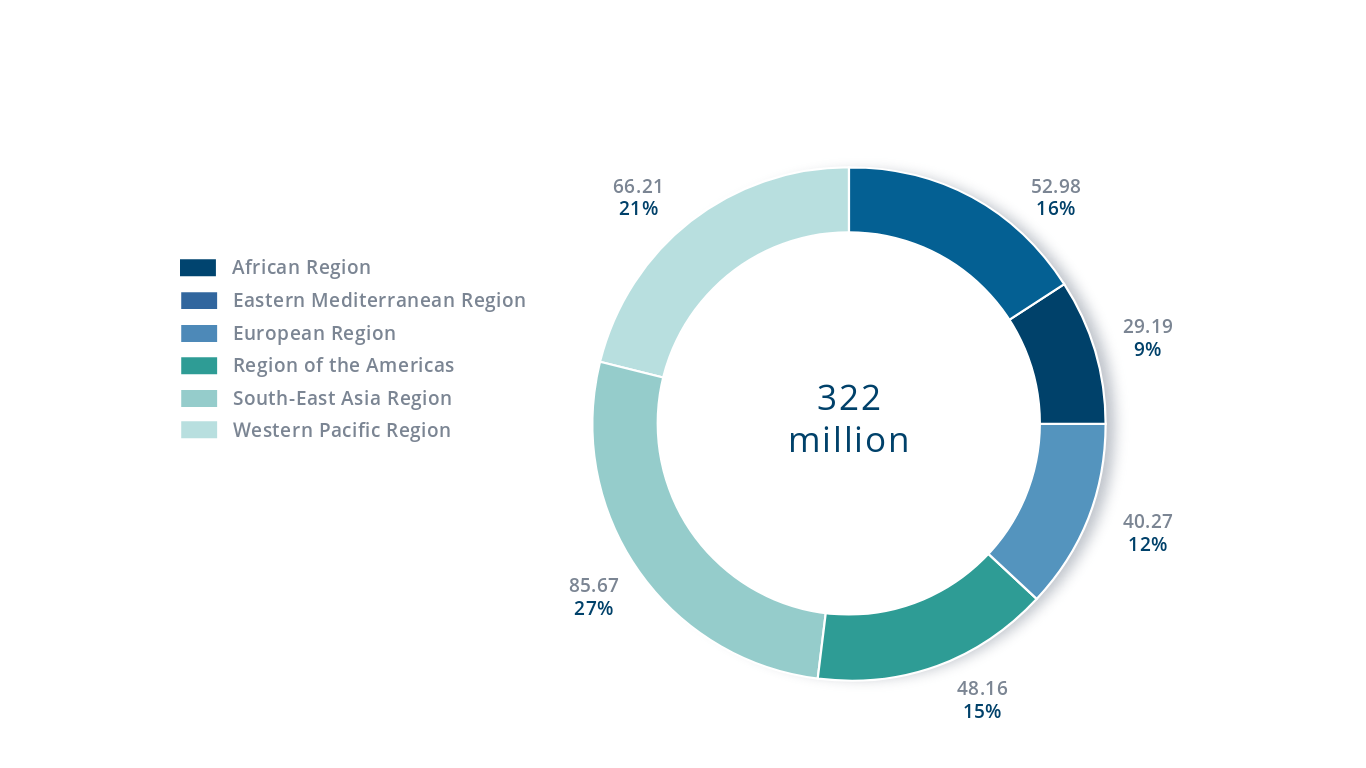
\includegraphics [scale=0.2]{images/stat_depression.png}
	\caption{Cases of depressive disorder by region in 2017 according to WHO. \cite{world2017depression}}
	\label{fig:stat_depression}
\end{figure}

Although there are clinical factors that can help in detecting patients at risk, some studies have shown that depressed people have particular linguistic expressions~\cite{FranceSSSW00,OzdasSSSW04,low2011detection}. For example, depressed people use more likely some specific linguistic patterns such as excessive use of personal pronouns, past tense or negative emotions. People'  writings can therefore be used as a cue to try to detect their psychological state and if they are possibly depressed.

In recent years, the emergence of social networks such as Facebook, Twitter or Reddit has allowed people to share their personal experiences, ideas or thoughts in a simpler way. According to the author in \cite{kulkarni2018early}, people actually prefer to express themselves online rather than offline. This phenomenon has generated a lot of data which is an opportunity for many research topics, and therefore also for the medical field~\cite{DallouxCCBG20}. In addition, a study by Marriott and Buchanan~\cite{marriott2014true} reports  there is no significant difference between an individual's online and offline personality in terms of authenticity. Social media is thus a good source for studying the ability of automatic system to help on the detection of depressed people. It becomes possible to study the writings of these users in order to try to detect depressed users based on linguistic indicators. 

Most approaches in the literature on detecting depression on social networks use supervised learning methods trained on manually annotated datasets. Different groups of features have been used such as the use of emoticons~\cite{WangZJSWB13}, the time of publication on the social network~\cite{Choudhury2013} and the themes mentioned~\cite{Resnik2015}. Different machine learning techniques can also be applicable to this type of problems, from well established categorization techniques to more recent deep learning models~\cite{Faneva20}. Nonetheless, these studies consider different data sets and there is no detailed analysis to compare different models and different types of features for early detection of depression.

Early depression detection implies that time is considered; the idea being to detect the early signals in the texts. Social media posts are generally time stamped and thus early detection is technically possible. The challenge then is to re-consider the models and features used for depression detection for the task  of early detection. Early detection means less information from each user to train the models; this may impact more some models than others. 


In this chapter, we present a supervised learning approach for early detection of depression. This work has been validated on the eRisk task datasets of the 2017 and 2018 editions presented in chapter~\ref{CH2}.
On the one hand,  we used well-established classifiers including logistic regression and random forest and on the other hand, we used the more recently developed BERT modeling~\cite{}. 
With the first type of models, we need to define the features that will be used in the vectors that will represent the information.  While we have re-used some features from the literature, we also consider new features in our models. BERT embeds the representation which is based on the texts, so that we do not need to define features but simply fine-tune the model on the specific problem to solve. Considering the impressive results of BERT-based models, we hypothesize that BERT will be better on the condition it has enough information to be fine-tuned while well establish models will better answer the problem of early detection.  
This chapter presents the multiple models we developed and evaluated on the task of depression detection and early depression detection. We also deeply analyze this results in order to provide useful insights on the advantages of the different versions of the models.

This chapter  is organized as follows: Section~\ref{CH4:soa} presents  features and models used to identify signs of depression from social media in related work.% \jm{Fabio said we need to include in this chapter all related work we think is relevant} \fr{relevant to us or relevant to E-Risk in general?} \jm{just for our chapter, thus for us}. 
Section~\ref{CH4:methods} details the data modeling, that is to say the features we use to build the models to be trained for early detection of depression. Section~\ref{CH4:results} presents the results on 2017 and 2018  eRisk challenge data sets. Section~\ref{CH4:ablation} is a deep analysis of the results to highlight the post important features. Section~\ref{CH4:Conclusion} concludes this chapter. 

\section{Related work}
Most of the work on the identification of depression in social media attempts to make the diagnosis process automatic. Much of this work is based on supervised learning methods and uses techniques such as statistical methods and natural language processing. 

Approaches based on statistical methods collect statistical elements by quantifying activity on social networking platforms, social isolation, number of friends, user network based on users' interests or mutual connections, etc. As for approaches that use natural language processing techniques, they are more based on linguistic/semantic analysis of posts such as analysis of emotions expressed, sentence structure, etc.


In the case of postpartum depression (a mood disorder that can affect mothers after childbirth), De Choudhury et al.~\cite{ChoudhuryCHH14} define several measures to characterize the differences between mothers with postpartum depression  and those without that they evaluated on  Facebook posts form 165 users from which 28 with PPD.  The authors define 49 characteristics that they grouped into 4 categories: \textit{user characteristics} which include characteristics that measure social network activity such as the number of posts per day, \textit{social capital} which includes measures on the interaction with others such as the number of mentions \textit{love} of friends' posts, \textit{content characteristics}  that are computed from the content of publications such as emotion analysis and \textit{linguistic style} that measure behavioral changes based on the use of linguistic styles in publications. The authors found that 35 of the 49 characteristics significantly (considering t-test) distinguish between the two groups. They developed several regression models to predict whether a mother is at risk for PPD. On the prenatal data, the model using all characteristics gives the best result, however, their best model overall is the one based on prenatal data combined with postnatal data. In our work, we were inspired or adapted some characteristics from their  \textit{content characteristics} and \textit{linguistic style} categories.

In another study, De Choudhury \textit{et al.} \cite{Choudhury2013} define several features and feature categories  to characterize Twitter users in relation to depression. The authors  crowdsourced 476 volonteer Twitter user' accounts of which 171 had a high CES-D\footnote{CES-D  stands for Center for Epidemiologic Studies Depression who provides a questionnaire that can be used to detect depression} score used as a cue for automatically detect depression. The authors defined 43 characteristics that they grouped into the following categories : \textit{engagement}, \textit{self-centered social graph (self-centered network)}, \textit{emotion}, \textit{language style} and \textit{depression language}. Four more demographic characteristics were considered : \textit{age}, \textit{gender}, \textit{level of education} and \textit{income}. The authors then analyzed the data  to try to distinguish between depressed and non-depressed behaviours. The authors found that those with depression engage in less social activity, display more negative emotions, pay more attention to themselves, show an increase in relational and medical concerns, and express more religious thoughts. They also found that even though their egocentric networks are small, depressed users appear to belong to closely grouped networks and are generally very connected to their network. De Choudhury \textit{et al.} also created several models, using different combinations of characteristics and different classification methods to predict whether a user is depressed or not based on their tweets. They found that the SVM classifier trained with features, reduced in size with the Principal Component Analysis (PCA) method, provided the best result with an accuracy of 70 \% and a precision of 0.74. In our work, we  adapted some of the characteristics from the groups \textit{emotion}, \textit{commitment} and \textit{depression language}.

The work carried in the e-Risk task (cf. Chapter \ref{CH2} of this book) are closer to ours than the ones from De Choudhury \textit{et al.}.  E-Risk differs from the above mentioned work in that its aims to detect as early as possible possible signs of depression  from users' texts, in this case Reddit~\footnote{Reddit is a social news aggregation, web content rating, and discussion website (\url{reddit.com})} forum posts. For early detection, the temporality is considered by dividing the set of chronologically ordered posts of a given user into 10 partitions containing 10\% of the user's texts each. Early depression detection hence is to predict whether a user is  depressed by using as few partitions as possible. Early detection is measured by ERDE$_{x}$ which has been defined  for the eRisk task (see section~\ref{CH2:measures} for more details) in addition to recall, precision and F1-measure.

Trotzek \textit{et al.} developed five models for early depression detection for E-Risk 2017. All these models use linguistic meta-information extracted from each user's texts and combine them with classifiers based on bag of words, paragraph vector, latent semantic analysis (LSA) and recurrent neural networks. Their bag of word model performed the best considering the F1-measure while their model based on  paragraph vectors performed best considering the precision and the ERDE$_{5}$. In E-Risk 2018, the same authors  used four machine learning models, two are based on convolutional neural network; the other two are based on features computed from the user's texts either considering bags of words or a combination of linguistic metadata and bags of words. They also considered an ensemble model that combines the results obtained from three (two models based on CNN and one features based model) of these four models~\cite{TrotzekKF18}. The
model that considers bags of words only performed the best  according to the ERDE$_{50}$ and F1-measure in 2018. They also obtained the best on the ERDE$_{5}$ and ERDE$_{50}$ on e-risk 2017 data set after the competition, %  \fr{après la campagne et mais sur erisk 17} 
 with another ensemble model which combines a CNN-based model using fastText as word embedding~\cite{GraveMJB17}  trained on Wikipedia articles and a model based on linguistic features~\cite{TrotzekKF20}. % \fr{No, they did not participate in E-Risk 2019 or 2020.}}.


Funez et al.~\cite{ErrecaldeVFUC17} proposed a model based on concise semantic analysis (CSA)~\cite{LI2011441}. CSA extracts a few concepts from category labels, here depressed vs non depressed. Each term is then represented as a vector in this concept space and a text or set of texts as the centroid of the  vectors terms it is composed of. This is used to represent each user considering his or her posts. For early depression detection, the authors considers the temporal difference of the representation of the users and named their model Temporal Variation of Terms (TVT) \jm{est-ce cela?}
 TVT model obtained the best performance for ERDE$_{5}$ and ERDE$_{50}$ measures on than stantard bag of words on E-risk 2017.
%proposed the Temporal Variation of Terms (TVT) method TVT. TVT is a document representation method based on the concise semantic analysis (CSA) technique but that includes temporality since it represents a document by using the variation of vocabulary along the different time steps. 
%\jm{c'est cela?}. %\jm{en quoi TVT n'est pas CSA alors? \fr{TVT utilise d'autres documents de la classe minoritaire pour la representation du nouveau document. C'est pour ça qu'elle s'accorde bie avec le problème de la détection au plutôt parce qu'elle va utiliser les textes des partition précédente. Elle arrive aussi le problème de données non balancées avec l'utilisation de documents précedents.}}. 
%CSA is a semantic analysis technique that 
% \fr{where a concept is close or equal to labels.} \jm{c'est quoi un label?  }. % that is equal or close to labels (classes) \jm{que voulez vous dire, je ne comprends pas. \fr{Je l'ai pris du papier original. Est ce qu'il faut aussi mettre leur exemple? ça permet de mieux comprendre parce que sinon c'est compliqué} \jm{ben il faut qu on comprenne}.
%CSA represents then a document as the centroid of the  vectors terms it is composed of. 
%\fr{TVT relies on the idea that variations of the terms used in the different sequential steps of the documents may contain information relevant to the classification} \jm{est ce que vous voulez dire dans les differents chunks? \fr{Oui ça peut être chunk pour eRisk mais d'autre documents pour d'autres tâches. C'est comme ça qu'il l'esplique dans leur papier. J'ai même peur que c'est un peu de plagiat tellement c'est difficile pour moi d'autres mots.} je ne comprends pas}. With this idea, TVT enriches the documents of the minority class \jm{c'est quoi? \fr{le moins nombreux label ou classe} \jm{c'est quoi ce lable ou classe dans le cas erisk?} with the partial documents read  in the first chunks (empirically 4 chunks in E-risk 2017) \jm{que voulez vous dire , est-ce simplement les docs des 4 premiers chunks? \fr{Je pense que c'est ça oui} autre chose "partial document read"??? \fr{Ben, c'est ce qui est écrit dans leur papier. Je pense que c'est les documents présent dans les 4 premier chunks}}. All this information \jm{de quoiparlez vous? et donc les concepts sont quoi?} is considered as a new concept of space for a CSA method.}

Later, Funez et al.~\cite{FunezUVBCME18} proposed a variant of TVT called FTVT (Flexible Temporal Variation of Terms) where the number of posts used is flexible. Their other model, SIC, incrementally reads documents and estimates the evidence that document's words provide depressive and/or non depressive labels. SIC classifies a user as depressive as soon as the accumulated evidence of the depressive class surpass the evidence of the other one.
%and also another method named SIC (sequential incremental classification). The difference between FTVT and TVT is that FTVT allows the specification of a different number of chunks \textit{n} for the distinct systems while it was fixed to 4 for TVT (JE NE SUIS PAS SUR SI C'EST VRAIMENT ça PARCE QUE LEUR EXPLICATION EST ASSEZ FLOU SUR LA DIFFERENCE.)

%\fr{SIC incrementally reads documents and estimates the evidence that document's words provide positive and/or negative labels. SIC classifies a user as positive as soon as the accumulated evidence of the positive class surpass the evidence of the negative one.} 
%proposed a model where documents are represented with concepts according to the Concise Semantic Analysis (CSA) approach. CSA represents terms as vectors in a concept space that is equal or close to labels (classes); and a document is the centroid of the term vectors that compose it. 
%The main idea of the TVT representation method is to use temporal information to obtain an extended concept space.  \jm{@Faneva, merci de ré-écrire tout cela, ce n'est pas très clair de comment cela fonctionne \fr{d'accord}}.
%This model improved the results they obtained using their prior model that was a combination of bags of words, words with the highest information gain and concepts considering the CSA approach \textit{et al.}~\cite{VillegasFUCE17,FunezUVBCME18} that they used in their participation to e-Risk in 2017 and 2018 and for which they obtained the best results for ERDE$_{50}$ measure (in 2017). Their versions of the system for 2018 edition \jm{@Faneva quels sont les changements entre TVT et FTVT?, c'est quoi SIC, cf texte ci dessous} 
%For the 2018 edition of the eRisk task, they proposed two different approaches: \ac{FTVT} which is an improvement of \ac{TVT}, and \ac{SIC}. 
For their participation to E-risk 2018, Funez et al.  submitted five models, three of which are variants from their FTVT approach (hyperparameter values are changed) from which one obtained the best ERDE$_{5}$, 
and two are variants from their SIC approach from which one obtained the best recall over the participants.
%\jm{did they continu in 2019 and later ? \fr{Yes but with SS3.}}


Burdisso \textit{et al.} \cite{BurdissoEM19} proposed the SS3 model which builds a dictionary of words, with their frequency, for each category \jm{c'est quoi la catégorie?}


SS3. The design of SS3 aims to address three main aspects of early detection problems: incremental classification of sequential data, support for early classification, and explicability. During the training phase and for each given category, SS3 builds a dictionary of words, with their frequency, for each category \jm{@Faneva et il fait cela à chaque chunk? c'est pour cela que c'est incrémental? ou pourquoi est-ce "incrémental?"}. Then, from these word frequencies, during the classification phase, SS3 calculates a value for each word using a $gv(w,c)$ function to evaluate the relationship between a $w$ word and a $c$ category. Then a vector version of $gv$, called a confidence vector, is defined: $\overrightarrow{gv(w)} = (gv(w,c_0),gv(w,c_1)$ where $c_i \in C$ and and $C$ is the set of all categories. For a classification, SS3 first divides the entry (e.g., documents or text) into blocks (e.g., paragraphs), then each block is further divided into smaller blocks until the words are reached. Then, SS3 calculates the $\overrightarrow{gv}$ confidence vector for each word, and then these confidence vectors are reduced using an operator (e.g., sum, maximum, etc.) to generate the confidence vectors for the upper block. This reduction process propagates recursively to the upper level blocks until only one confidence vector is generated for the input. Finally, the classification is performed on the basis of the values of this single confidence vector (e.g. by selecting the category with the highest confidence value). They tested SS3 to solve the problem to be addressed by the eRisk 2017 task. They obtained the best result by considering the ERDE$_{5}$ measure against the participants of the task. In the same work, they proposed SS3$^{\bigtriangleup}$, which is different from SS3 on classification policy. With SS3$^{\bigtriangleup}$, they got the best result considering the ERDE$_{50}$ measure in relation to the participants of the eRisk 2017 task. 
Burdisso \textit{et al.} extended their approach 
s the SS3 approach \cite{BurdissoEM19} and proposes $\tau-$SS3 \cite{BurdissoEM19B}. $\tau-$SS3 dynamically recognizes useful patterns/patterns on text streams, i.e. it can learn and recognize N-grams of variable length. This new method has been tested on both eRisk task editions (2017 and 2018) on depression detection and has provided better results than SS3. Compared to the results of other participants, $\tau-$SS3 performed best considering the ERDE$_{5}$ and ERDE$_{50}$ measures on the 2017 edition and best considering the ERDE$_{50}$ measure on the 2018 edition. \jm{je dois revoir une fois les réponses à mes questions données}


\jm{@Faneva, au final, il y a beaucoup de best... peut être un tableau permettrait de s'y retrouver, en fonction de l'année et de la mesure ...\fr{d'accor, je vais faire un tableau}}

\fr{In the table, I took the best result for each measure in the paper, It means that the results are from different models. Should I details the models in table instead? \jm{I think you should have a line for each model in the Table, yes, In the first column you could name the models differently than in the initial paper if you want. and also add \cite{} rather than the name of the team. }}
\begin{table}[]
    \centering
    \caption{List of models in the literature and their results in the eRisk Dataset.}
    \label{tab:state_of_art}
    \begin{tabular}{|l|c|c|c|c|c|c|c|c|c|c|}
        \hline
         \multirow{2}{*}{Models}&\multicolumn{5}{c|}{2017} & \multicolumn{5}{c|}{2018} \\
         \cline{2-11}
         & ERDE$_{5}$ & ERDE$_{50}$ & F1-measure & Precision & Recall & ERDE$_{5}$ & ERDE$_{50}$ & F1-measure & Precision & Recall \\
         \hline
        Trotzek & 12.70 \% & 9.69 \% & 0.64 & 0.69 & 0.67& 9.21 \%& 6.44 & 0.64 & 0.64 & 0.72  \\
        %FHDOA & 12.82 \% & 9.69 \% & 0.64 & 0.61 & 0.67& & & & &  \\
        UArizona & 13.07 \% & 10.23 \% & 0.45 & 0.34 & 0.92& & - & - & - & - \\
        UNSL & 13.66 \% & 9.68 \% & 0.59 & 0.48 & 0.79& 8.78& 6.95&0.60 & 0.53&  0.85\\\hline
        SS3 & 12.60 \% & 8.12 \% & 0.52 & 0.44 & 0.63& & & & &  \\
        $\tau-$SS3 & 12.60 \% & 7.70 \% & 0.55 & 0.43 & 0.77&9.48 \% & 6.17 \% & - & - & -\\
        \hline
    \end{tabular}
\end{table}

\jm{bonjour Faneva. concernant la depression, vous avez travaillé juste sur 2017 et 2018? \fr{oui}
et y a t il des données sur d'autres années ? \fr{oui, j'ai les données des années 2020 et 2019, mais pour ces années c'est sur l'anorexie, self-harm et la mesure de la gravité des signes de dépression (et la detection simple de la dépression).}}

\jm{du coup, si on a du temps, on peut essayer la detection simple de la depression sur 2019 et 2020 (pendant la période de relecture des articles par exemple) \fr{d'accord}}



---------------

\section{Information modeling}
For depression detection, the objective is to detect whether a user is predicted to be depressed giving her or his posts. For early depression detection, the objective is close to the previous one, but the detection should be based on a minimum of posts considering their chronological order. To solve these problems, we rely on machine learning techniques which principle is to learn a decision from a set of examples for which the decision is known. In the case of depression detection, an example is a user described by a list of features and the label is binary indicating whether the user is depressed. 

Considering e-risk data, we have no information on the users for anonymity reasons, which is often the case when considering personal data, but we know their posts. User features have thus to be extracted from a series of user's posts, either all the posts for depression detection, or a sub-part of them for early depression detection. To extract the users' features, we considered two approaches: feature-based and word embedding based. We  then successively use the two representations on well-establish machine learning algorithms (see Sub-section\ref{CH4:xx}) to 


% the With regards to the models, we considered both well-established machine learning models and more recent BERT modeling. For each of them we describe the key points that also make these approaches re-usable in other contexts.




\subsection{Feature-based representation}
\label{CH4:sec:sub:featurerepresentation}

%All feature, different ML models
%then we keep the best for meta-ablation study (6 models)

The features we considered are many (252 in total). They come both from the  literature~\cite{Choudhury2013,ChoudhuryCHH14} or from our own developments
\jm{@Faneva, pouvez vous ajouter les références nécessaires ici?}

We categorized these features into five meta-categories (meta1 to meta5) each of which are  divided in turn into categories (numbered with roman numeral I to XVI). This hierarchical representation of features will be used for deep analysis of the impact of features on the results. 
The five meta-categories are as follows: representation of full texts, lexicons on depression, temporal aspects, writing style,  and emotion. These meta-categories, the associated categories and features are detailed in Table~\ref{CH4:tab:features}. 

\jm{Table is in Table.tex}
\jm{@Zia, we do not manage to handle this Table, could you try?}\zu{Ok}
%The problem is here: caption and label should be in one line end with '\\' "\caption{Description of the features used to represent the information. Similar type of features are grouped.}\label{CH4:tab:features}\\"

\jm{can we lower the size of the font in the table? (in one command, not for each text to avoid errors} \zu{Yes, we can do this. I use "footnotesize", may be we can use "small" size also}
\jm{@Faneva: complétez un peu les références et il y a des phrases non finies, que le lecteur ait suffisament d'infor pour refaire s'il le souhaite}  
\jm{@Faneva rajouter aussi les références utiles}


%\lowercase{}
%\begin{center}
% \begin{longtable}{@{} l@{\hspace{.2em}} l@{\hspace{.2em}} p{3.3cm} @{\hspace{.2em}} @{\hspace{.2em}} p{6cm}} 
% \caption{Description of the features used to represent the information. Similar type of features are grouped.}
%\label{CH4:tab:features}\\

%\hline
%Group & Number & Name & Hypothesis or tool$-$resource used\\
%\hline
% \end{longtable}
%\end{center}
%\begin{center}
\begin{longtable}{@{} l@{\hspace{.2em}} l@{\hspace{.2em}} p{3.3cm} @{\hspace{.2em}} @{\hspace{.2em}} p{6cm}} 
\caption{Description of the features used to represent the information. Similar type of features are grouped.}\label{CH4:tab:features}\\
\hline
Group & Number & Name & Hypothesis or tool/resource used\\
\hline
\endfirsthead
%Group & \# & Name & & Hypothesis or tool/resource used\\
\endhead
\multicolumn{4}{c}{\scshape{Meta$_{1}$}: Representation of full texts}\\
\hline
 I & 1-18 & Bag of words & $18$ most frequent uni-grams in the training set.\\[3pt]
\hline
II & 19-22 & Part-Of-Speech frequency & Higher usage of adjectives, verbs and adverbs and lower usage of nouns.\\[3pt]
\hline
\multirow{3}{*}{III}
& 45 & Depression symptoms and related drugs & From Wikipedia list and ~\cite{Choudhury2013}\\
& 48 & Relevant 3-grams & 25 3-grams described from.\\
& 49 & Relevant 5-grams & 25 5-grams described from.\\[3pt]
\hline
\multicolumn{4}{c}{\scshape{Meta$_{2}$}: Lexicons on depression}\\
\hline
IV & 47 & Frequency of ``depress" & Depressed people talk often about the depression.\\[3pt]
\hline
V & 58 & {Drugs name} & The chemical and brand names of antidepressants from WebMD available in United States.\\[3pt]
\hline
\multicolumn{4}{c}{\scshape{Meta$_{3}$}:Temporality}\\
\hline
\multirow{2}{*}{VI}
& 43 & Temporal expressions & High use of words that refer to past: last,before,ago, ....\\
& 46 & Sleepy Words & Depressive users talk more about their sleeping.\\[3pt]
\hline
\multirow{2}{*}{VII}
& 50 & Ratio of Posting Time & High frequency of publications in deep night (00 pm - 07 am).\\
& 253-256 & Season of a year (4 seasons in total) & {Frequency of publications in season (one season corresponds to 3 months).}\\[3pt]
\hline
\multirow{3}{*}{VIII}
& 41 & Past frequency & Combination of temporal expressions and past tense verbs.\\
& 42 & Past tense verbs & Depressive people talk more about the past.\\
& 44 & Past tense auxiliaries & Same motivation as above.\\[3pt]
\hline
\multicolumn{4}{c}{\scshape{Meta$_{4}$}: Writing style}\\
\hline
\multirow{5}{*}{IX} 
& 27 & Average number of posts & Depressed users have a much lower number of posts.\\
& 28 & Average number of words per post & Posts of depressed user are more longer.\\
& 29 & Minimum number of posts & Generally depressive users have a lower value.\\
& 30 & Average number of comments & Depressed users have a much lower number of comments.\\
& 31 & Average number of words per comment & Comments of depressed and non depressed users have different means.\\[3pt]
\hline
%\pagebreak
\multirow{4}{*}{X}
& 54 & Gunning Fog Index & Estimate of the years of education that a person needs to understand the text at first reading.\\ 
& 55 & Flesch Reading Ease & Measure how difficult to understand a text is.\\
& 56 & Linsear Write Formula & Developed for the U.S. Air Force to calculate the readability of their technical manuals.\\
& 57 & New Dale-Chall Readability & Measure the difficulty of comprehension that persons encounter when reading a text. It is inspired from Flesch Reading Ease measure.\\[3pt]
\hline
\multirow{4}{*}{XI} 
& 32-36 & First person pronouns & High use of : \textit{I, me, myself, mine, my}.\\
& 37 &\textit{I} subject of \textit{be} & High use of \textit{I'm}.\\
& 38 & All first person pronouns & Sum of frequency of each first pronoun .\\
& 39 & \textit{I} in subjective context & Depressive users refers to themselves frequently (all \textit{I} targeted by an adjective).\\[3pt]
\hline
XII & 40 & Over-generalization  & Depressed users tend to use intense quantifiers and {superlatives}.\\[3pt]
\hline
XIII & 23 & Negation & Depressive users use more negative words like: \textit{no, not, didn’t, can't}, ...., etc. \\[3pt]
\hline
\multirow{3}{*}{XIV}
& 24 & Capitalized & Depressive users tend to put emphasis on the target they mention.\\
& 26 & Punctuation marks & ! or ? or any combination of both tend to express doubt and surprise.\\
& 53 & Emotions & Frequency of emotions from specific categories: anger, fear, surprise, sadness and disgust.\\[3pt]
\hline
\multicolumn{4}{c}{\scshape{Meta$_{5}$}: Emotion}\\
\hline
\multirow{2}{*}{XV}
& 25 & Emoticons & Another way to express sentiment or feeling.\\
& 51-52 & Sentiment & Use of NRC-Sentiment-Emotion-Lexicons to trace the polarity in users writings.\\
\hline
XVI & 59-252 & Empathy & all 194 empathy categories\\ 
\hline
\end{longtable}
\end{center}
\begin{center}
\begin{footnotesize}
\begin{longtable}{@{} l@{\hspace{.2em}} l@{\hspace{.2em}} p{3.3cm} @{\hspace{.2em}} @{\hspace{.2em}} p{6cm}} 
\caption{Description of the features used to represent the information. Similar type of features are grouped.}\label{CH4:tab:features}\\
\hline
Group & Number & Name & Hypothesis or tool/resource used\\
\hline
\endfirsthead
%Group & \# & Name & & Hypothesis or tool/resource used\\
\endhead
\multicolumn{4}{c}{\scshape{Meta$_{1}$}: Representation of full texts}\\
\hline
 I & 1-18 & Bag of words & $18$ most frequent uni-grams in the training set.\\[3pt]
\hline
II & 19-22 & Part-Of-Speech frequency & Higher usage of adjectives, verbs and adverbs and lower usage of nouns.\\[3pt]
\hline
\multirow{3}{*}{III}
& 45 & Depression symptoms and related drugs & From Wikipedia list and ~\cite{Choudhury2013}\\
& 48 & Relevant 3-grams & 25 3-grams described from.\\
& 49 & Relevant 5-grams & 25 5-grams described from.\\[3pt]
\hline
\multicolumn{4}{c}{\scshape{Meta$_{2}$}: Lexicons on depression}\\
\hline
IV & 47 & Frequency of ``depress" & Depressed people talk often about the depression.\\[3pt]
\hline
V & 58 & {Drugs name} & The chemical and brand names of antidepressants from WebMD available in United States.\\[3pt]
\hline
\multicolumn{4}{c}{\scshape{Meta$_{3}$}:Temporality}\\
\hline
\multirow{2}{*}{VI}
& 43 & Temporal expressions & High use of words that refer to past: last,before,ago, ....\\
& 46 & Sleepy Words & Depressive users talk more about their sleeping.\\[3pt]
\hline
\multirow{2}{*}{VII}
& 50 & Ratio of Posting Time & High frequency of publications in deep night (00 pm - 07 am).\\
& 253-256 & Season of a year (4 seasons in total) & {Frequency of publications in season (one season corresponds to 3 months).}\\[3pt]
\hline
\multirow{3}{*}{VIII}
& 41 & Past frequency & Combination of temporal expressions and past tense verbs.\\
& 42 & Past tense verbs & Depressive people talk more about the past.\\
& 44 & Past tense auxiliaries & Same motivation as above.\\[3pt]
\hline
\multicolumn{4}{c}{\scshape{Meta$_{4}$}: Writing style}\\
\hline
\multirow{5}{*}{IX} 
& 27 & Average number of posts & Depressed users have a much lower number of posts.\\
& 28 & Average number of words per post & Posts of depressed user are more longer.\\
& 29 & Minimum number of posts & Generally depressive users have a lower value.\\
& 30 & Average number of comments & Depressed users have a much lower number of comments.\\
& 31 & Average number of words per comment & Comments of depressed and non depressed users have different means.\\[3pt]
\hline
%\pagebreak
\multirow{4}{*}{X}
& 54 & Gunning Fog Index & Estimate of the years of education that a person needs to understand the text at first reading.\\ 
& 55 & Flesch Reading Ease & Measure how difficult to understand a text is.\\
& 56 & Linsear Write Formula & Developed for the U.S. Air Force to calculate the readability of their technical manuals.\\
& 57 & New Dale-Chall Readability & Measure the difficulty of comprehension that persons encounter when reading a text. It is inspired from Flesch Reading Ease measure.\\[3pt]
\hline
\multirow{4}{*}{XI} 
& 32-36 & First person pronouns & High use of : \textit{I, me, myself, mine, my}.\\
& 37 &\textit{I} subject of \textit{be} & High use of \textit{I'm}.\\
& 38 & All first person pronouns & Sum of frequency of each first pronoun .\\
& 39 & \textit{I} in subjective context & Depressive users refers to themselves frequently (all \textit{I} targeted by an adjective).\\[3pt]
\hline
XII & 40 & Over-generalization  & Depressed users tend to use intense quantifiers and {superlatives}.\\[3pt]
\hline
XIII & 23 & Negation & Depressive users use more negative words like: \textit{no, not, didn’t, can't}, ...., etc. \\[3pt]
\hline
\multirow{3}{*}{XIV}
& 24 & Capitalized & Depressive users tend to put emphasis on the target they mention.\\
& 26 & Punctuation marks & ! or ? or any combination of both tend to express doubt and surprise.\\
& 53 & Emotions & Frequency of emotions from specific categories: anger, fear, surprise, sadness and disgust.\\[3pt]
\hline
\multicolumn{4}{c}{\scshape{Meta$_{5}$}: Emotion}\\
\hline
\multirow{2}{*}{XV}
& 25 & Emoticons & Another way to express sentiment or feeling.\\
& 51-52 & Sentiment & Use of NRC-Sentiment-Emotion-Lexicons to trace the polarity in users writings.\\
\hline
XVI & 59-252 & Empathy & all 194 empathy categories\\ 
\hline
\end{longtable}
\end{footnotesize}
\end{center}

\subsubsection{Word embedding  representation}
As in~\ref{CH4:sec:sub:featurerepresentation}, each user is represented by a vector built from his or her posts but here we use embeddings at the sentence level. First we calculate a sentence embedding vector for each post, then for a given user, we aggregate all the vectors from that user's posts by averaging the vectors; we thus calculate the centroid vector for each user. 

In this work, we will use the Doc2Vec quote{LeM14} sentence plunge which is based on the Word2Vec quote{mikolov2013distributed} word plunge presented in Chapter \ref{CH2:}. The concept is simple: add another vector (paragraph id) to the Word2vec template (see figure \ref{fig:architecture_d2v}). The goal of Doc2vec is to create a digital representation of a document/text, whatever its length. Doc2vec can work very well when trained on a small corpus compared to Word2vec \cite{trotzeklinguistic}. 

\begin{figure}[!ht]
	%\centering
	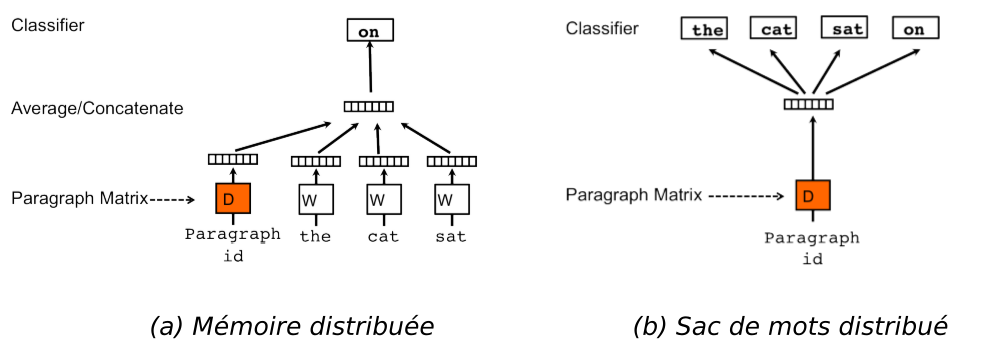
\includegraphics[scale=0.4]{images/architecture_doc2vec.png}
	\caption{Doc2Vec models~\cite{LeM14} \jm{@faneva, traduire dans la figure}}
	\label{fig:architecture_d2v}
\end{figure}

\jm{@Faneva: pouvez vous decrire ici ce dont on a besoin, c'est à dire ce qui a été utilisé dans les experimentations}

\section{Machine learning models}
\subsection{Well-established machine learning models}

\jm{the models we used need to be described RF, LR, SVM\_RBF, SVM\_Linear, Neural network, KNN}


However, these classical classifiers are not designed to solve detection problems at the earliest possible time while we deal with such problems in this work. Early detection problems integrate a time dimension in the classification, in other words, they use data streams as input. That is, at a given instant t, only a partition of the data is available for classification and the further forward in time, the more data is available. The objective is to have the best results using the minimum amount of data, i.e. as quickly as possible over time. 

To allow classical classifiers to deal with the problem we face in this work, we adopt a classification process where we integrate the time dimension outside the classifiers. This process consists first of all in training classifiers without taking into account the time dimension, in other words, using all the data available in the training corpus. Second, we use these trained classifiers for the earliest possible detection of depression on the test data. Specifically, at a given time t and for a given user, a classifier classifies the user using only the data available at that time. If the user is classified as depressed then the classification process stops, otherwise the classifier classifies the user again using the data available at time t+1. This process is repeated and at the end, if the user is still not classified by the classifier as depressed, then the user is considered to be non-depressed.

\subsection{Bert-based model}
BERT (Bidirectional Encoder Representations from Transformers) is a pre-training language representation model. Bert model architecture is a multi-layer bidirectional transformer encoder, which considers both left and right context in all layers. BERT is pre-trained on large corpus using the so called masking technique: given a sentence, 15\% of the input words are masked and during training, the goal is to predict these words. This technique overcomes the limitation of unidirectional processing and is also superior to language models that combine right-to-left and left-to-right processing, see  \cite{PetersNIGCLZ18}.  Pre-trained  Google BERTs are freely available on github\footnote{\url{https://github.com/google-research/bert}, accessed February 02, 2021}. The BERT$_{Base}$ model contains 12 layers of size 768, 12 self-attention heads and 110M parameters, while the BERT$_{Large}$ model contains 24 layers of size 1,024, 16 self-attention heads and 340M parameters. BERT can be fine-tuned to answer specific tasks.

In this work, we used the BERT$_{Base}$ model that we fine tuned \jm{@Zia....by???.}




\subsection{x}
\section{Evaluation}

\jm{Do not include e-risk description, Fabio said there is a specific chapter on that. What is written here, you can keep, but rather focus on our work , not on their work}

\subsection{Experimental plans}
description du plan d'experience et des objectifs\\
description of the experience plan and objectives

\subsection{Collections}
CLEF e-Risk 2017 and 2018 collections.

\begin{table}[!ht]
    \caption{Distribution of training and test data from the eRisk 2017 and 2018 collection on depression task.}
    \centering
    \begin{tabular}{|l@{\hspace*{0.2cm}}|l@{\hspace*{0.2cm}}| l@{\hspace*{0.1cm}}| r@{\hspace*{0.2cm}}| r@{\hspace*{0.2cm}}| r@{}|}
	%\begin{tabular}{|c|m{3.5cm}|c|c||c|c|}
		\hline
		\multicolumn{2}{|c|}{\multirow{2}{*}{Number}} &	\multicolumn{2}{c|}{Training} & \multicolumn{2}{c|}{Test}\\
		\cline{3-6} \multicolumn{2}{|c|}{} & Depressive & Non-depressive & Depressive & Non-depressive\\
		\hline
		\multirow{3}{*}{2017} & Users &	83 & 403 & 52 & 349\\ 
		\cline{2-6}
		& Posts	& 4,911 & 91,381 & 1,928 & 65,735\\
		\cline{2-6}
		& Comments & 25,940	& 172,791 & 16,778 & 151,930\\
		\cline{2-6} 
		\hline
		\multirow{3}{*}{2018} & Users & 135 & 752 & 79 & 741\\
		\cline{2-6}
		& Posts	& 6,839 & 157,116 &  7,672	& 169,930\\
		\cline{2-6}	& Comments & 42,718 &  324,721 & 32,993 & 333,852\\ 
		\hline 
	\end{tabular}\label{CH4:tab:dataset}
\end{table}

\subsection{Measures}
For early depression detection, a new measure has been defined (see Chapter~\ref{CH2:}. This new measurement takes into account the accuracy of the decisions made by the system, but also the time it takes to issue this decision. This measure is called \textit{early risk detection error} (\emph{ERDE}) and was defined by Losada \textit{et al.}\cite{losada2017erisk} as follows: 
%{\small
	\begin{equation}\label{eq:ERDE_mesure}
    	ERDE_{o}(d,k) = 
	    \left\{
	        \begin{matrix}
	            c_{fp} & if $\;d = positive\;$ and $\;gt = negative$\\ 
	            c_{fn} & if $\;d = negative\;$ and $\;gt = positive$\\ 
	            lc_{o}(k)\cdot c_{tp} & if $\;d = positive\;$ and $\;gt = positive$\\ 
            	0 & if $\;d = negative\;$ and $\;gt = negative$\\
	        \end{matrix}
	    \right.
	\end{equation}
%}
where $gt$ denotes the ground truth, $c_{tp}$, $c_{fn}$, $c_{fp}$, and $lc_{o}(k)$ are defined as follows:

\begin{itemize}
	\item $c_{fn} = c_{tp} = 1$,
	\item $c_{fp}$ is the proportion of positive cases in test data,
	\item $lc_{o}(k) = 1 - \frac{1}{1+e^{k-o}}$,
	\item $o$ is a parameter which equals to 5 and 50 for ERDE$_{5}$ and ERDE$_{50}$, respectively.
\end{itemize}

Note that the ERDE value of a method is the average of the ERDE calculated for each user using Equation~\ref{eq:ERDE_mesure}. Also, the smaller the value of the ERDE measurement, the better the method.

We also considered other standard measures used to evaluate classification methods such as Precision (P), Recall (R), and F1-measure (F). 

\begin{equation}
    F = 2 \times \frac{R \times P}{R + P}
\end{equation}


\section{Results and discussion}

\jm{\subsection{Experiments : @Faneva or Zia:}}
\begin{enumerate}
  
    \item \jm{ I think it would be interesting to also have a decision based on all the data, at the end. We could add a section on that. Where both BERT, word embeedings with various ML and all features with various ML would be compared} \zu{All features with various ML is done.}\zu{Word embedding with various ML is continuing and then BERT}
    \item \jm{then, we could renew this comparison, but for earlt detection, at various chuncks}
    \item \jm{then we will have the ablation study}
\end{enumerate}

\jm{we could compare Bert and classical ML; I think it could be interesting because Bert may need more information than traditional, thus early detection may be better with traditional, while binary decision without early detection may be better with Bert. }


\begin{table}[h!]
\caption{\textit{Well-Established machine learning methods using the 256 features} for eRisk 2017 and 2018 collections considering all the  features listed Table~\ref{CH4:tab:features}. Threshold on predicted probability is 0.5.}
{
\centering
\resizebox{0.7\textwidth}{!}{
\begin{tabular}{@{}l@{\hspace{.5em}}|l@{\hspace{.5em}}|c@{\hspace{.5em}}c@{\hspace{.5em}}c@{\hspace{.5em}} r@{\hspace{.5em}} r@{}}
& ML model & $P$ & $R$ & $F_{1}$ & $ERDE_{5}$ & $ERDE_{50}$\\
\hline
\multirow{6}{*}{\rotatebox[origin=c]{270}{2017}}
& RF & .63 & .62 & .62 & 12.71\% & 9.48\%\\
& LR & .21 & .88 & .34 & 16.82\% & 11.39\\
& SVM ($rbf$)\\
& SVM ($linear$)\\
& NN\\
& KNN\\
\hline
\multirow{6}{*}{\rotatebox[origin=c]{270}{2018}}
& RF & .65 & .53 & .58 & 9.41\% & 7.19\%\\
& LR & .16 & .84 & .27 & 11.94\% & 8.84\%\\
& SVM ($rbf$)\\
& SVM ($linear$)\\
& NN\\
& KNN\\
\hline
\end{tabular}}\label{CH4:tab:erisk_overall}}
\end{table}

\subsection{Depression detection}
In this section, we present the results for depression detection, that is to say without considering its early detection. From the set of user's posts, the system has to predict whether the user is depressed. We thus train the models on the training set and run the obtained model on the entire test set, without considering chunks or partitions.

Table~\ref{CH2:tab:xx} presents the results where machine learning uses (a)  the 256 features and well-established ML algorithms (RF, LR, SVM\_RBF, SVM\_Linear, Neural network, KNN) \jm{all these models have to be presented} (b) word embeddings  with the same well-established ML algorithms (c) BERT 

\jm{thus here, it would not be early detection, but just detection. We could use the 4 years here. No ERDE measure thus because we train on the training (entire). }

\jm{@Faneva, is that possible or not? }

\subsection{Early depression detection}

\subsection{Simplified models}
\jm{@Faneva, c'est les modèles avec juste les features les plus importants Ki2: pouvez vous présenter le principe de simplification et les résultats obtenus (cf thèse)}

\subsection{Ablation analysis}
In the ablation analysis, we considered random forest  with feature-based models. On the one hand we consider the reference model, the one that uses all the 256 features, to which we remove some features (exclusion); on the other hand, we consider models where a limited set of features  are considered (inclusion). We conduced the analysis at the meta level as well as at the category level.


\subsubsection{Meta level analysis}
In the \textit{exclusion analysis}, from the reference model (first row, Table~\ref{CH4:tab:erisk_ablation_meta}), we removed one meta category of features, considering successively each of the five meta categories. This approach helps in understanding which are the less and most influencing meta categories. If the results decrease when removing a meta category of features, that means that the corresponding features are important. 
In the \textit{inclusion analysis}, we build a model that contains the features of a single meta category each time.

From Table~\ref{CH4:tab:erisk_ablation_meta}, we can see that the model that includes all the features is among the best for both collections. Each measure aims at providing different insights on the model capability. Recall and precision are inversely related while F1-measure combines recall and precision. When focusing on F1-measure, we can observe that excluding {\scshape Meta$_{5}$} (emoticons) is not consistently problematic: it is for 2017 data set, where both recall and precision decrease, but not for the 2018 data set where precision only decreases but recall increases. Overall, when considering F1-measure, recall and precision, removing one of the meta categories does not affect much the results. This shows that the features from the different category have some kind of redundancy although there are not of the same nature. The same type of conclusion can be drown when analyzing the early detection measures.  {\scshape Meta$_{5}$} (emoticons) does not help much early detection: when removed (Exclusion), the results are improved. We can also see that in general not considering the full text representation  (Exclusion {\scshape Meta$_{1}$}) hurts the results the most, for almost all the measures. That means that focused features such as lexicons, writing style, emoticons, etc. are not enough, still the entire text is useful.

Now when considering a limited number of features (Inclusion), we can see that some meta categories are  more helpful than others and that they can be complementary. For example, {\scshape Meta$_{3}$} (\jm{xx}) features help for  recall for both collections but are not enough to obtain acceptable precision. On the other hand, {\scshape Meta$_{1}$} features are key for early detection (lowest ERDE for the model that uses these features) while {\scshape Meta$_{3}$}  features are not (high ERDE).


\begin{table}[h!]
\caption{Ablation study of the meta group of features both in exclusion and inclusion strategy using the Random forest (RF) classifier. Threshold on predicted probability is 0.5.}{
\centering
%\zu{There is another related one from 2019: "Task 3: Measuring the severity of the signs of depression"} \fr{I have the dataset if you want. this Task 3 was a little bit different.}\zu{Ok} \jm{I think this is another task, let us focus on the task Faneva participated to. Rather, thus, now the BERT results could be added}


\resizebox{1.0\textwidth}{!}{
\begin{tabular}{@{} l@{\hspace{.2em}} | l@{\hspace{.25em}} | c@{\hspace{.25em}} c@{\hspace{.25em}} c@{\hspace{.25em}} r@{\hspace{.25em}} r@{\hspace{.25em}} | c@{\hspace{.25em}} c@{\hspace{.25em}} c@{\hspace{.25em}} r@{\hspace{.25em}} r@{}|}
\hline
& Features & \multicolumn{5}{c|}{Exclusion} & \multicolumn{5}{c|}{Inclusion}\\
\hline
& & $P$ & $R$ & $F_1$ & \small{$ERDE_5$}& $ERDE_{50}$ & $P$ & $R$ & $F_1$ & $ERDE_5$ & $ERDE_{50}$\\
\hline
\multirow{6}{*}{\rotatebox[origin=c]{270}{2017}}
&All & .63 & \textbf{.62 }& \textbf{.62} & 12.71\% &\textbf{ 9.48}\% & \textbf{.63} & \textbf{.62} & \textbf{.62} & 12.71\% & \textbf{9.48}\%\\[2pt]
& \hspace*{.03cm} - {\scshape Meta$_{1}$} & .63 & .56 & .59 & 13.01\% & 9.91\% & .54 & .52 & .53 & \textbf{12.65}\% & 9.72\%\\
& \hspace*{.03cm} - {\scshape Meta$_{2}$} & .62 & .56 & .59 & 12.68\% & 9.44\% & .58 & .58 & .58 & 13.37\% & 11.43\%\\
& \hspace*{.03cm} - {\scshape Meta$_{3}$} & .66 & .56 & .60 & 12.59\% & 9.84\% & .13 & \textbf{.62} & .21 & 18.22\% & 14.94\%\\
& \hspace*{.03cm} - {\scshape Meta$_{4}$} & \textbf{.68} & .58 & \textbf{.62} & 12.99\% & 9.58\% & .27 & .60 & .37 & 14.35\% & 11.65\%\\
& \hspace*{.03cm} - {\scshape Meta$_{5}$} & .55 & .54 & .54 & \textbf{12.50}\% & 9.97\% & .62 & .58 & .60 & 13.40\% & 10.19\%\\
\hline
\multirow{6}{*}{\rotatebox[origin=c]{270}{2018}}
&All & \textbf{.65} & .53 & .58 & 9.41\% & 7.19\% & \textbf{.65 }& .53 &\textbf{ .58} & \textbf{9.41}\% & 7.19\%\\[2pt]
& \hspace*{.03cm} - {\scshape Meta$_{1}$} & .63 & .54 & \textbf{.59} & 9.58\% & 6.88\% & .54 & .46 & .49 & 9.45\% &\textbf{ 6.95}\%\\
& \hspace*{.03cm} - {\scshape Meta$_{2}$} & .58 & .53 & .56 & 9.44\% & 6.82\% & .34 & \textbf{.65} & .45 & 10.13\% & 8.22\%\\
& \hspace*{.03cm} - {\scshape Meta$_{3}$} & .66 & .53 & \textbf{.59} & 9.50\% & \textbf{6.72}\% & .10 & .62 & .17 & 13.47\% & 11.11\%\\
& \hspace*{.03cm} - {\scshape Meta$_{4}$} & \textbf{.65} & .51 & .57 & 9.48\% & 7.09\% & .20 & .54 & .29 & 10.25\% & 7.74\%\\
& \hspace*{.03cm} - {\scshape Meta$_{5}$} & .60 & \textbf{.58} & \textbf{.59} & \textbf{9.17}\% & 6.92\% & .62 & .51 & .56 & 9.77\% & 7.36\%\\
\hline
\end{tabular}}\label{CH4:tab:erisk_ablation_meta}}
\end{table}




\subsubsection{Category level analysis}

\begin{table}[t]
\caption{Ablation study of the category of features defined in Table~\ref{CH4:tab:features} considering both exclusion and inclusion strategy using the Random forest classifier. Threshold on predicted probability is 0.5.}{
\centering
\resizebox{.90\textwidth}{!}{
\begin{tabular}{@{} l@{\hspace{.2em}} | l@{\hspace{.35em}} | c@{\hspace{.35em}} c@{\hspace{.35em}} c@{\hspace{.35em}} r@{\hspace{.35em}} r@{\hspace{.35em}} | c@{\hspace{.35em}} c@{\hspace{.35em}} c@{\hspace{.35em}} r@{\hspace{.35em}} r@{}|}
\hline
& Features & \multicolumn{5}{c|}{Exclusion} & \multicolumn{5}{c|}{Inclusion}\\
\hline
& & $P$ & $R$ & $F_1$ & $ERDE_5$& $ERDE_{50}$ & $P$ & $R$ & $F_1$ & $ERDE_5$ & $ERDE_{50}$\\
\hline
\multirow{6}{*}{\rotatebox[origin=c]{270}{2017}}
& All & .63 & .62 & .62 & 12.71\% & 9.48\% & .63 & .62 & .62 & 12.71\% & 9.48\%\\[2pt]
& \hspace*{.003cm} - {\scshape I} & .62 & .54 & .58 & 12.97\% & 10.09\% & .47 & .54 & .50 & 13.17\% & 9.98\%\\
& \hspace*{.003cm} - {\scshape II} & .70 & .62 & .65 & 12.72\% & 9.37\% & .38 & .58 & .46 & 13.86\% & 10.12\%\\
& \hspace*{.003cm} - {\scshape III} & .66 & .60 & .63 & 12.80\% & 9.87\% & .18 & .52 & .27 & 15.85\% & 13.14\%\\
& \hspace*{.003cm} - {\scshape IV} & .64 & .56 & .60 & 13.02\% & 9.37\% & .47 & .54 & .50 & 13.74\% & 11.48\%\\
& \hspace*{.003cm} - {\scshape V} & .62 & .56 & .59 & 12.70\% & 10.13\% & .55 & .12 & .19 & 13.13\% & 12.63\%\\
& \hspace*{.003cm} - {\scshape VI} & .69 & .65 & .67 & 12.65\% & 9.59\% & .28 & .37 & .32 & 13.88\% & 10.78\%\\
& \hspace*{.003cm} - {\scshape VII} & .65 & .62 & .63 & 12.72\% & 9.41\% & .13 & .73 & .23 & 18.88\% & 10.62\%\\
& \hspace*{.003cm} - {\scshape VIII} & .62 & .58 & .60 & 12.69\% & 9.93\% & .25 & .65 & .36 & 14.17\% & 10.99\%\\
& \hspace*{.003cm} - {\scshape IX} & .64 & .58 & .61 & 12.82\% & 9.66\% & .14 & .90 & .24 & 21.66\% & 10.24\%\\
& \hspace*{.003cm} - {\scshape X} & .70 & .62 & .65 & 12.55\% & 9.25\% & .25 & .56 & .34 & 14.59\% & 11.94\%\\
& \hspace*{.003cm} - {\scshape XI} & .66 & .56 & .60 & 12.58\% & 9.41\% & .41 & .52 & .46 & 14.17\% & 11.73\%\\
& \hspace*{.003cm} - {\scshape XII} & .65 & .62 & .63 & 12.84\% & 9.22\% & .14 & .90 & .24 & 21.66\% & 17.54\%\\
& \hspace*{.003cm} - {\scshape XIII} & .66 & .60 & .63 & 12.61\% & 10.12\% & .15 & .83 & .25 & 20.73\% & 17.62\%\\
& \hspace*{.003cm} - {\scshape XIV} & .65 & .62 & .63 & 12.83\% & 9.41\% & .24 & .44 & .31 & 14.54\% & 11.90\%\\
& \hspace*{.003cm} - {\scshape XV} & .62 & .58 & .60 & 12.69\% & 9.44\% & .16 & .27 & .20 & 15.31\% & 13.65\%\\
& \hspace*{.003cm} - {\scshape XVI} & .60 & .58 & .59 & 12.81\% & 10.12\% & .70 & .62 & .65 & 12.80\% & 9.19\%\\
\hline
\multirow{6}{*}{\rotatebox[origin=c]{270}{2018}}
& All & .65 & .53 & .58 & 9.41\% & 7.19\% & .65 & .53 & .58 & 9.41\% & 7.19\%\\[2pt]
& \hspace*{.003cm} - {\scshape I} & .59 & .49 & .54 & 9.15\% & 7.02\% & .50 & .46 & .48 & 9.70\% & 7.25\%\\
& \hspace*{.003cm} - {\scshape II} & .65 & .52 & .58 & 9.34\% & 6.84\% & .29 & .44 & .35 & 9.82\% & 7.41\%\\
& \hspace*{.003cm} - {\scshape III} & .60 & .56 & .58 & 9.39\% & 6.82\% & .17 & .63 & .27 & 11.88\% & 9.83\%\\
& \hspace*{.003cm} - {\scshape IV} & .57 & .52 & .54 & 9.49\% & 6.83\% & .42 & .57 & .48 & 10.07\% & 8.09\%\\
& \hspace*{.003cm} - {\scshape V} & .60 & .51 & .55 & 9.49\% & 6.66\% & .47 & .28 & .35 & 9.89\% & 9.32\%\\
& \hspace*{.003cm} - {\scshape VI} & .60 & .51 & .55 & 9.55\% & 6.90\% & .21 & .39 & .27 & 10.28\% & 8.42\%\\
& \hspace*{.003cm} - {\scshape VII} & .71 & .49 & .58 & 9.53\% & 7.02\% & .09 & .68 & .16 & 14.40\% & 11.79\%\\
& \hspace*{.003cm} - {\scshape VIII} & .58 & .51 & .54 & 9.40\% & 7.17\% & .23 & .57 & .33 & 10.73\% & 8.71\%\\
& \hspace*{.003cm} - {\scshape IX} & .65 & .51 & .57 & 9.58\% & 7.33\% & .16 & .41 & .23 & 10.39\% & 8.73\%\\
& \hspace*{.003cm} - {\scshape X} & .66 & .53 & .59 & 9.38\% & 6.97\% & .22 & .52 & .31 & 10.23\% & 8.07\%\\
& \hspace*{.003cm} - {\scshape XI} & .62 & .53 & .57 & 9.34\% & 7.17\% & .37 & .49 & .42 & 9.81\% & 7.61\%\\
& \hspace*{.003cm} - {\scshape XII} & .60 & .52 & .56 & 9.56\% & 6.78\% & .10 & .76 & .18 & 15.61\% & 13.29\%\\
& \hspace*{.003cm} - {\scshape XIII} & .60 & .53 & .56 & 9.44\% & 6.79\% & .10 & .80 & .18 & 15.59\% & 13.36\%\\
& \hspace*{.003cm} - {\scshape XIV} & .61 & .52 & .56 & 9.46\% & 6.89\% & .23 & .44 & .31 & 10.37\% & 9.04\%\\
& \hspace*{.003cm} - {\scshape XV} & .59 & .51 & .54 & 9.34\% & 6.91\% & .15 & .25 & .19 & 10.94\% & 9.96\%\\
& \hspace*{.003cm} - {\scshape XVI} & .60 & .63 & .61 & 9.12\% & 6.74\% & .59 & .49 & .54 & 9.76\% & 7.15\%\\
\hline
\end{tabular}}\label{CH4:tab:erisk_ablation_group}}
\end{table}

When considering the exclusion of a category of features, we can see that part-of-speech features (II) could be omitted -either the results are improved like on 2017 or they are stable like on 2018 data. The results are consistently better when omitting the category (X) of readability features. 

\section{Transfer to other health-related domains}

\section{Conclusion}

\section{References}

\newpage

\section{Section Heading}
\label{sec:1}
Use the template \emph{chapter.tex} together with the document class SVMono (monograph-type books) or SVMult (edited books) to style the various elements of your chapter content.

Instead of simply listing headings of different levels we recommend to let every heading be followed by at least a short passage of text.  Further on please use the \LaTeX\ automatism for all your cross-references and citations. And please note that the first line of text that follows a heading is not indented, whereas the first lines of all subsequent paragraphs are.

\section{Section Heading}
\label{sec:2}
% Always give a unique label
% and use \ref{<label>} for cross-references
% and \cite{<label>} for bibliographic references
% use \sectionmark{}
% to alter or adjust the section heading in the running head
Instead of simply listing headings of different levels we recommend to let every heading be followed by at least a short passage of text.  Further on please use the \LaTeX\ automatism for all your cross-references and citations.

Please note that the first line of text that follows a heading is not indented, whereas the first lines of all subsequent paragraphs are.

Use the standard \verb|equation| environment to typeset your equations, e.g.
%
\begin{equation}
a \times b = c\;,
\end{equation}
%
however, for multiline equations we recommend to use the \verb|eqnarray| environment\footnote{In physics texts please activate the class option \texttt{vecphys} to depict your vectors in \textbf{\itshape boldface-italic} type - as is customary for a wide range of physical subjects}.
\begin{eqnarray}
\left|\nabla U_{\alpha}^{\mu}(y)\right| &\le&\frac1{d-\alpha}\int
\left|\nabla\frac1{|\xi-y|^{d-\alpha}}\right|\,d\mu(\xi) =
\int \frac1{|\xi-y|^{d-\alpha+1}} \,d\mu(\xi)  \\
&=&(d-\alpha+1) \int\limits_{d(y)}^\infty
\frac{\mu(B(y,r))}{r^{d-\alpha+2}}\,dr \le (d-\alpha+1)
\int\limits_{d(y)}^\infty \frac{r^{d-\alpha}}{r^{d-\alpha+2}}\,dr
\label{eq:01}
\end{eqnarray}

\subsection{Subsection Heading}
\label{subsec:2}
Instead of simply listing headings of different levels we recommend to let every heading be followed by at least a short passage of text.  Further on please use the \LaTeX\ automatism for all your cross-references\index{cross-references} and citations\index{citations} as has already been described in Sect.~\ref{sec:2}.

\begin{quotation}
Please do not use quotation marks when quoting texts! Simply use the \verb|quotation| environment -- it will automatically be rendered in line with the preferred layout.
\end{quotation}


\subsubsection{Subsubsection Heading}
Instead of simply listing headings of different levels we recommend to let every heading be followed by at least a short passage of text.  Further on please use the \LaTeX\ automatism for all your cross-references and citations as has already been described in Sect.~\ref{subsec:2}, see also Fig.~\ref{fig:1}\footnote{If you copy text passages, figures, or tables from other works, you must obtain \textit{permission} from the copyright holder (usually the original publisher). Please enclose the signed permission with the manuscript. The sources\index{permission to print} must be acknowledged either in the captions, as footnotes or in a separate section of the book.}

Please note that the first line of text that follows a heading is not indented, whereas the first lines of all subsequent paragraphs are.

% For figures use
%
\begin{figure}[b]
\sidecaption
% Use the relevant command for your figure-insertion program
% to insert the figure file.
% For example, with the graphicx style use
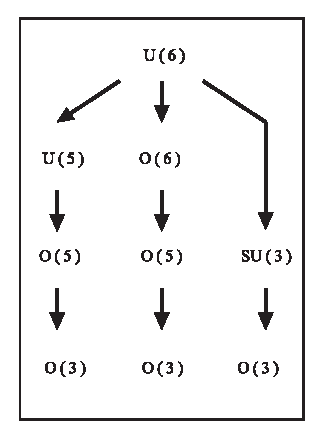
\includegraphics[scale=.65]{figure}
%
% If no graphics program available, insert a blank space i.e. use
%\picplace{5cm}{2cm} % Give the correct figure height and width in cm
%
\caption{If the width of the figure is less than 7.8 cm use the \texttt{sidecapion} command to flush the caption on the left side of the page. If the figure is positioned at the top of the page, align the sidecaption with the top of the figure -- to achieve this you simply need to use the optional argument \texttt{[t]} with the \texttt{sidecaption} command}
\label{fig:1}       % Give a unique label
\end{figure}


\paragraph{Paragraph Heading} %
Instead of simply listing headings of different levels we recommend to let every heading be followed by at least a short passage of text.  Further on please use the \LaTeX\ automatism for all your cross-references and citations as has already been described in Sect.~\ref{sec:2}.

Please note that the first line of text that follows a heading is not indented, whereas the first lines of all subsequent paragraphs are.

For typesetting numbered lists we recommend to use the \verb|enumerate| environment -- it will automatically rendered in line with the preferred layout.

\begin{enumerate}
\item{Livelihood and survival mobility are oftentimes coutcomes of uneven socioeconomic development.}
\begin{enumerate}
\item{Livelihood and survival mobility are oftentimes coutcomes of uneven socioeconomic development.}
\item{Livelihood and survival mobility are oftentimes coutcomes of uneven socioeconomic development.}
\end{enumerate}
\item{Livelihood and survival mobility are oftentimes coutcomes of uneven socioeconomic development.}
\end{enumerate}


\subparagraph{Subparagraph Heading} In order to avoid simply listing headings of different levels we recommend to let every heading be followed by at least a short passage of text. Use the \LaTeX\ automatism for all your cross-references and citations as has already been described in Sect.~\ref{sec:2}, see also Fig.~\ref{fig:2}.

For unnumbered list we recommend to use the \verb|itemize| environment -- it will automatically be rendered in line with the preferred layout.

\begin{itemize}
\item{Livelihood and survival mobility are oftentimes coutcomes of uneven socioeconomic development, cf. Table~\ref{tab:1}.}
\begin{itemize}
\item{Livelihood and survival mobility are oftentimes coutcomes of uneven socioeconomic development.}
\item{Livelihood and survival mobility are oftentimes coutcomes of uneven socioeconomic development.}
\end{itemize}
\item{Livelihood and survival mobility are oftentimes coutcomes of uneven socioeconomic development.}
\end{itemize}

\begin{figure}[t]
\sidecaption[t]
% Use the relevant command for your figure-insertion program
% to insert the figure file.
% For example, with the option graphics use
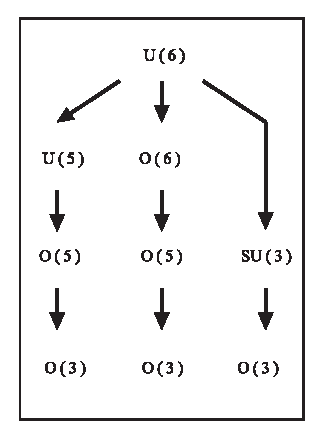
\includegraphics[scale=.65]{figure}
%
% If no graphics program available, insert a blank space i.e. use
%\picplace{5cm}{2cm} % Give the correct figure height and width in cm
%
%\caption{Please write your figure caption here}
\caption{If the width of the figure is less than 7.8 cm use the \texttt{sidecapion} command to flush the caption on the left side of the page. If the figure is positioned at the top of the page, align the sidecaption with the top of the figure -- to achieve this you simply need to use the optional argument \texttt{[t]} with the \texttt{sidecaption} command}
\label{fig:2}       % Give a unique label
\end{figure}

\runinhead{Run-in Heading Boldface Version} Use the \LaTeX\ automatism for all your cross-references and citations as has already been described in Sect.~\ref{sec:2}.

\subruninhead{Run-in Heading Boldface and Italic Version} Use the \LaTeX\ automatism for all your cross-refer\-ences and citations as has already been described in Sect.~\ref{sec:2}\index{paragraph}.

\subsubruninhead{Run-in Heading Displayed Version} Use the \LaTeX\ automatism for all your cross-refer\-ences and citations as has already been described in Sect.~\ref{sec:2}\index{paragraph}.
% Use the \index{} command to code your index words
%
% For tables use
%
\begin{table}[!t]
\caption{Please write your table caption here}
\label{tab:1}       % Give a unique label
%
% Follow this input for your own table layout
%
\begin{tabular}{p{2cm}p{2.4cm}p{2cm}p{4.9cm}}
\hline\noalign{\smallskip}
Classes & Subclass & Length & Action Mechanism  \\
\noalign{\smallskip}\svhline\noalign{\smallskip}
Translation & mRNA$^a$  & 22 (19--25) & Translation repression, mRNA cleavage\\
Translation & mRNA cleavage & 21 & mRNA cleavage\\
Translation & mRNA  & 21--22 & mRNA cleavage\\
Translation & mRNA  & 24--26 & Histone and DNA Modification\\
\noalign{\smallskip}\hline\noalign{\smallskip}
\end{tabular}
$^a$ Table foot note (with superscript)
\end{table}
%
\section{Section Heading}
\label{sec:3}
% Always give a unique label
% and use \ref{<label>} for cross-references
% and \cite{<label>} for bibliographic references
% use \sectionmark{}
% to alter or adjust the section heading in the running head
Instead of simply listing headings of different levels we recommend to let every heading be followed by at least a short passage of text.  Further on please use the \LaTeX\ automatism for all your cross-references and citations as has already been described in Sect.~\ref{sec:2}.

Please note that the first line of text that follows a heading is not indented, whereas the first lines of all subsequent paragraphs are.

If you want to list definitions or the like we recommend to use the enhanced \verb|description| environment -- it will automatically rendered in line with the preferred layout.

\begin{description}[Type 1]
\item[Type 1]{That addresses central themes pertainng to migration, health, and disease. In Sect.~\ref{sec:1}, Wilson discusses the role of human migration in infectious disease distributions and patterns.}
\item[Type 2]{That addresses central themes pertainng to migration, health, and disease. In Sect.~\ref{subsec:2}, Wilson discusses the role of human migration in infectious disease distributions and patterns.}
\end{description}

\subsection{Subsection Heading} %
In order to avoid simply listing headings of different levels we recommend to let every heading be followed by at least a short passage of text. Use the \LaTeX\ automatism for all your cross-references and citations citations as has already been described in Sect.~\ref{sec:2}.

Please note that the first line of text that follows a heading is not indented, whereas the first lines of all subsequent paragraphs are.

\begin{svgraybox}
If you want to emphasize complete paragraphs of texts we recommend to use the newly defined class option \verb|graybox| and the newly defined environment \verb|svgraybox|. This will produce a 15 percent screened box 'behind' your text.

If you want to emphasize complete paragraphs of texts we recommend to use the newly defined class option and environment \verb|svgraybox|. This will produce a 15 percent screened box 'behind' your text.
\end{svgraybox}


\subsubsection{Subsubsection Heading}
Instead of simply listing headings of different levels we recommend to let every heading be followed by at least a short passage of text.  Further on please use the \LaTeX\ automatism for all your cross-references and citations as has already been described in Sect.~\ref{sec:2}.

Please note that the first line of text that follows a heading is not indented, whereas the first lines of all subsequent paragraphs are.

\begin{theorem}
Theorem text goes here.
\end{theorem}
%
% or
%
\begin{definition}
Definition text goes here.
\end{definition}

\begin{proof}
%\smartqed
Proof text goes here.
%\qed
\end{proof}

\paragraph{Paragraph Heading} %
Instead of simply listing headings of different levels we recommend to let every heading be followed by at least a short passage of text.  Further on please use the \LaTeX\ automatism for all your cross-references and citations as has already been described in Sect.~\ref{sec:2}.

Note that the first line of text that follows a heading is not indented, whereas the first lines of all subsequent paragraphs are.
%
% For built-in environments use
%
\begin{theorem}
Theorem text goes here.
\end{theorem}
%
\begin{definition}
Definition text goes here.
\end{definition}
%
\begin{proof}
%\smartqed
Proof text goes here.
%\qed
\end{proof}
%
\begin{trailer}{Trailer Head}
If you want to emphasize complete paragraphs of texts in an \verb|Trailer Head| we recommend to
use  \begin{verbatim}\begin{trailer}{Trailer Head}
...
\end{trailer}\end{verbatim}
\end{trailer}
%
\begin{question}{Questions}
If you want to emphasize complete paragraphs of texts in an \verb|Questions| we recommend to
use  \begin{verbatim}\begin{question}{Questions}
...
\end{question}\end{verbatim}
\end{question}
\eject%
\begin{important}{Important}
If you want to emphasize complete paragraphs of texts in an \verb|Important| we recommend to
use  \begin{verbatim}\begin{important}{Important}
...
\end{important}\end{verbatim}
\end{important}
%
\begin{warning}{Attention}
If you want to emphasize complete paragraphs of texts in an \verb|Attention| we recommend to
use  \begin{verbatim}\begin{warning}{Attention}
...
\end{warning}\end{verbatim}
\end{warning}

\begin{programcode}{Program Code}
If you want to emphasize complete paragraphs of texts in an \verb|Program Code| we recommend to
use

\verb|\begin{programcode}{Program Code}|

\verb|\begin{verbatim}...\end{verbatim}|

\verb|\end{programcode}|

\end{programcode}
%
\begin{tips}{Tips}
If you want to emphasize complete paragraphs of texts in an \verb|Tips| we recommend to
use  \begin{verbatim}\begin{tips}{Tips}
...
\end{tips}\end{verbatim}
\end{tips}
\eject
%
\begin{overview}{Overview}
If you want to emphasize complete paragraphs of texts in an \verb|Overview| we recommend to
use  \begin{verbatim}\begin{overview}{Overview}
...
\end{overview}\end{verbatim}
\end{overview}
\begin{backgroundinformation}{Background Information}
If you want to emphasize complete paragraphs of texts in an \verb|Background|
\verb|Information| we recommend to
use

\verb|\begin{backgroundinformation}{Background Information}|

\verb|...|

\verb|\end{backgroundinformation}|
\end{backgroundinformation}
\begin{legaltext}{Legal Text}
If you want to emphasize complete paragraphs of texts in an \verb|Legal Text| we recommend to
use  \begin{verbatim}\begin{legaltext}{Legal Text}
...
\end{legaltext}\end{verbatim}
\end{legaltext}
%
\begin{acknowledgement}
If you want to include acknowledgments of assistance and the like at the end of an individual chapter please use the \verb|acknowledgement| environment -- it will automatically be rendered in line with the preferred layout.
\end{acknowledgement}
%
\section*{Appendix}
\addcontentsline{toc}{section}{Appendix}
%
%
When placed at the end of a chapter or contribution (as opposed to at the end of the book), the numbering of tables, figures, and equations in the appendix section continues on from that in the main text. Hence please \textit{do not} use the \verb|appendix| command when writing an appendix at the end of your chapter or contribution. If there is only one the appendix is designated ``Appendix'', or ``Appendix 1'', or ``Appendix 2'', etc. if there is more than one.

\begin{equation}
a \times b = c
\end{equation}


%@inproceedings{ChoudhuryCHH14,
	author    = {Munmun De Choudhury and
	Scott Counts and
	Eric Horvitz and
	Aaron Hoff},
	title     = {Characterizing and predicting postpartum depression from shared facebook
	data},
	booktitle = {Computer Supported Cooperative Work, {CSCW} '14, Baltimore, MD, USA,
	February 15-19, 2014},
	pages     = {626--638},
	year      = {2014},
	url       = {https://doi.org/10.1145/2531602.2531675},
	doi       = {10.1145/2531602.2531675},
	timestamp = {Tue, 06 Nov 2018 16:57:12 +0100},
	biburl    = {https://dblp.org/rec/bib/conf/cscw/ChoudhuryCHH14},
	bibsource = {dblp computer science bibliography, https://dblp.org}
}

@PhDThesis{Faneva2020,
	title={Extraction et fouille de données textuelles: application à ladétection de la dépression, de l'anorexie et de l'agressivité dans les réseaux sociaux},
   author={Iarivony Faneva, RAMIANDRISOA},
   school={Université de Toulouse},
	year={2020}
}

@inproceedings{Resnik2015,
	author    = {Philip Resnik and
	William Armstrong and
	Leonardo Max Batista Claudino and
	Thang Nguyen and
	Viet{-}An Nguyen and
	Jordan L. Boyd{-}Graber},
	title     = {Beyond {LDA:} Exploring Supervised Topic Modeling for Depression-Related
	Language in {Twitter}},
	booktitle = {Proceedings of CLPsych@NAACL-HLT}, 
	year      = {2015},
	url       = {http://aclweb.org/anthology/W/W15/W15-1212.pdf},
	timestamp = {Wed, 14 Sep 2016 10:01:11 +0200},
	biburl    = {http://dblp.org/rec/bib/conf/naacl/ResnikACNNB15},
	bibsource = {dblp computer science bibliography, http://dblp.org}
}

@inproceedings{Choudhury2013,
	author    = {Munmun De Choudhury and
	Michael Gamon and
	Scott Counts and
	Eric Horvitz},
	title     = {Predicting Depression via Social Media},
	booktitle = {Proceedings of the Seventh International Conference on Weblogs and
	Social Media}, 
	year      = {2013},
	url       = {http://www.aaai.org/ocs/index.php/ICWSM/ICWSM13/paper/view/6124},
	timestamp = {Tue, 20 Aug 2013 13:12:33 +0200},
	biburl    = {http://dblp.org/rec/bib/conf/icwsm/ChoudhuryGCH13},
	bibsource = {dblp computer science bibliography, http://dblp.org}
}

@inproceedings{Schwartz2014,
	author    = {H. Andrew Schwartz and
	Johannes C. Eichstaedt and
	Margaret L. Kern and
	Gregory J. Park and
	Maarten Sap and
	David Stillwell and
	Michal Kosinski and
	Lyle H. Ungar},
	title     = {Towards assessing changes in degree of depression through Facebook},
	booktitle={Proceedings of the Workshop on Computational Linguistics and Clinical Psychology: From Linguistic Signal to Clinical Reality}, 
	pages={118--125},
	year      = {2014}
}

@inproceedings{WangZJSWB13,
	author    = {Xinyu Wang and
	Chunhong Zhang and
	Yang Ji and
	Li Sun and
	Leijia Wu and
	Zhana Bao},
	title     = {A Depression Detection Model Based on Sentiment Analysis in Micro-blog
	Social Network},
	booktitle = {Trends and Applications in Knowledge Discovery and Data Mining - {PAKDD}
	2013 International Workshops: DMApps, DANTH, QIMIE, BDM, CDA, CloudSD,
	Gold Coast, QLD, Australia, April 14-17, 2013, Revised Selected Papers},
	pages     = {201--213},
	year      = {2013},
	url       = {https://doi.org/10.1007/978-3-642-40319-4\_18},
	doi       = {10.1007/978-3-642-40319-4\_18},
	timestamp = {Wed, 04 Jul 2018 00:35:03 +0200},
	biburl    = {https://dblp.org/rec/bib/conf/pakdd/WangZJSWB13},
	bibsource = {dblp computer science bibliography, https://dblp.org}
}

@article{marriott2014true,
	author    = {Tamsin C. Marriott and
	Tom Buchanan},
	title     = {The true self online: Personality correlates of preference for self-expression
	online, and observer ratings of personality online and offline},
	journal   = {Computers in Human Behavior},
	volume    = {32},
	pages     = {171--177},
	year      = {2014},
	url       = {https://doi.org/10.1016/j.chb.2013.11.014},
	doi       = {10.1016/j.chb.2013.11.014},
	timestamp = {Sat, 20 May 2017 00:23:41 +0200},
	biburl    = {https://dblp.org/rec/bib/journals/chb/MarriottB14},
	bibsource = {dblp computer science bibliography, https://dblp.org}
}

@inproceedings{DallouxCCBG20,
  author    = {Cl{\'{e}}ment Dalloux and
               Vincent Claveau and
               Marc Cuggia and
               Guillaume Bouzill{\'{e}} and
               Natalia Grabar},
  title     = {Supervised Learning for the {ICD-10} Coding of French Clinical Narratives},
  booktitle = {Digital Personalized Health and Medicine - Proceedings of {MIE} 2020,
               Medical Informatics Europe, Geneva, Switzerland, April 28 - May 1,
               2020},
  pages     = {427--431},
  year      = {2020},
  url       = {https://doi.org/10.3233/SHTI200196},
  doi       = {10.3233/SHTI200196},
  timestamp = {Thu, 13 Aug 2020 18:46:36 +0200},
  biburl    = {https://dblp.org/rec/conf/mie/DallouxCCBG20.bib},
  bibsource = {dblp computer science bibliography, https://dblp.org}
}

@article{FranceSSSW00,
	author    = {Daniel J. France and
	Richard G. Shiavi and
	Stephen E. Silverman and
	Marilyn K. Silverman and
	D. Mitchell Wilkes},
	title     = {Acoustical properties of speech as indicators of depression and suicidal
	risk},
	journal   = {{IEEE} Trans. Biomed. Engineering},
	volume    = {47},
	number    = {7},
	pages     = {829--837},
	year      = {2000},
	url       = {https://doi.org/10.1109/10.846676},
	doi       = {10.1109/10.846676},
	timestamp = {Sat, 27 May 2017 14:24:59 +0200},
	biburl    = {https://dblp.org/rec/bib/journals/tbe/FranceSSSW00},
	bibsource = {dblp computer science bibliography, https://dblp.org}
}

@article{low2011detection,
	author    = {Lu{-}Shih Alex Low and
	Namunu C. Maddage and
	Margaret Lech and
	Lisa Sheeber and
	Nicholas B. Allen},
	title     = {Detection of Clinical Depression in Adolescents' Speech During Family
	Interactions},
	journal   = {{IEEE} Trans. Biomed. Engineering},
	volume    = {58},
	number    = {3},
	pages     = {574--586},
	year      = {2011},
	url       = {https://doi.org/10.1109/TBME.2010.2091640},
	doi       = {10.1109/TBME.2010.2091640},
	timestamp = {Wed, 14 Nov 2018 10:16:28 +0100},
	biburl    = {https://dblp.org/rec/bib/journals/tbe/LowMLSA11},
	bibsource = {dblp computer science bibliography, https://dblp.org}
}

@article{OzdasSSSW04,
	author    = {Asli Ozdas and
	Richard G. Shiavi and
	Stephen E. Silverman and
	Marilyn K. Silverman and
	D. Mitchell Wilkes},
	title     = {Investigation of vocal jitter and glottal flow spectrum as possible
	cues for depression and near-term suicidal risk},
	journal   = {{IEEE} Trans. Biomed. Engineering},
	volume    = {51},
	number    = {9},
	pages     = {1530--1540},
	year      = {2004},
	url       = {https://doi.org/10.1109/TBME.2004.827544},
	doi       = {10.1109/TBME.2004.827544},
	timestamp = {Wed, 14 Nov 2018 10:16:19 +0100},
	biburl    = {https://dblp.org/rec/bib/journals/tbe/OzdasSSSW04},
	bibsource = {dblp computer science bibliography, https://dblp.org}
}

@MastersThesis{kulkarni2018early,
	title={Early Detection of Depression},
   author={Kulkarni, Akshay Bhavani Kumar},
   school={University of Houston},
	year={2018}
}

@inproceedings{losada2017erisk,
  title={eRISK 2017: CLEF lab on early risk prediction on the internet: experimental foundations},
  author={Losada, David E and Crestani, Fabio and Parapar, Javier},
  booktitle={International Conference of the Cross-Language Evaluation Forum for European Languages},
  pages={346--360},
  year={2017},
  organization={Springer}
}

@article{LI2011441,
title = {Fast text categorization using concise semantic analysis},
journal = {Pattern Recognition Letters},
volume = {32},
number = {3},
pages = {441-448},
year = {2011},
issn = {0167-8655},
doi = {https://doi.org/10.1016/j.patrec.2010.11.001},
url = {https://www.sciencedirect.com/science/article/pii/S0167865510003582},
author = {Zhixing Li and Zhongyang Xiong and Yufang Zhang and Chunyong Liu and Kuan Li},
}


\bibliography{ChapterMothe} 

\end{document}
